\section{Design}
The system was made on top of a plywood base plate with a tablecloth. The layout consisted of four zones. Closest to onlookers, a serving station was placed. Here, finished waffles would lie in wait of mouths to feed. Next to it was the preperation zone. Here a batter bowl and grease was placed. Right behind the preperation zone lied the waffle iron. The waffle iron had a custom set of rod inserts that would be baked into the waffles, allowing for easy extraction when they were done. In the opposite corner, the electronics needed to drive the hardware was placed. These electronics were placed in a protective housing, shown in figure \ref{fig:mechanical}. The housing had a lid, on top of which the robot was placed. Each of the mechanical components had special modifications made that made it easier for the robot to interact with its environment.
\vskip1cm
\begin{figure}[h]
    \centering
    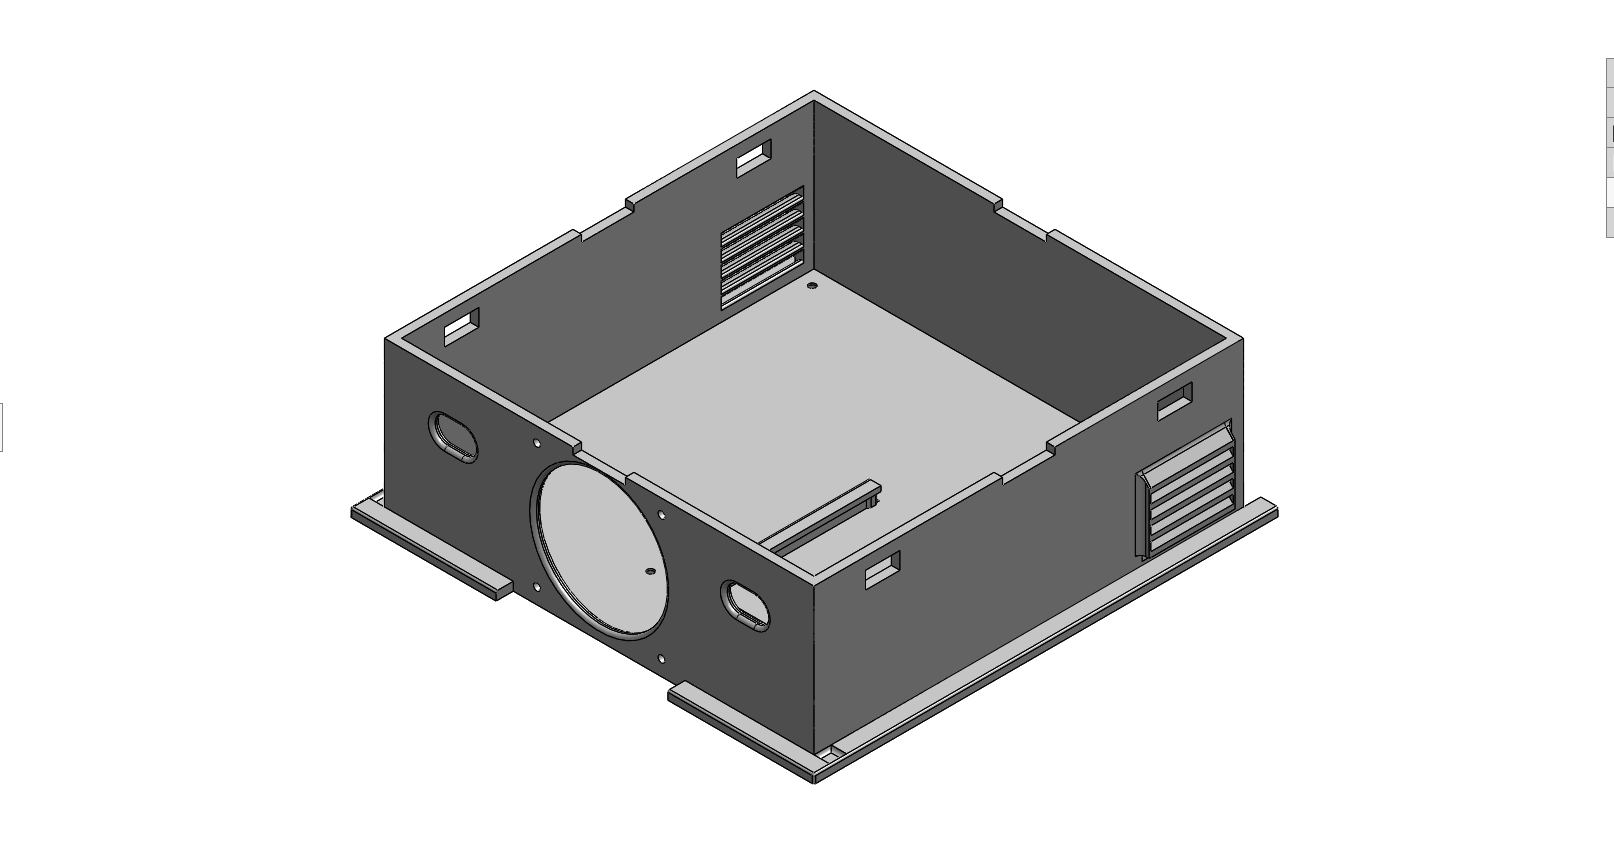
\includegraphics[width= 1\linewidth]{figures/boxv3.png}
    \caption{The housing used to mount electronics.}
    \label{fig:mechanical}
\end{figure}
The control software used was based on the principle of moving the robot by hand and recording its positions. When the record button was pressed, the camera would simultanously take a picture. Each object of relevance had an ArUco marker attatched to itself. Image processing was used to find the positions of the marker. The position of the marker would be referenced against the position of the robot to record the relative pose from marker to robot. The offsets were computed using equation \eqref{eq:offset_from_marker} and played back later with \eqref{eq:arm_from_marker}.
\begin{align}
    \mathbf{O} &= \mathbf{M}^{-1}\mathbf{A}\label{eq:offset_from_marker}\\
    \mathbf{A} &= \mathbf{M}\mathbf{O} \label{eq:arm_from_marker}
\end{align}
 This setup allowed the robot to follow along with the marker if it moved.  The concept is shown in figure \ref{fig:badExample}. 

\begin{figure}[h]
    \centering
    \includesvg[width= 1\linewidth]{figures/tagoffsets.svg}
    \caption{Concept of recording the offset O with a marker M and arm position A.}
    \label{fig:badExample}
\end{figure}
This technology was also repurposed to create an alternate activity for the robot to perform when it was waiting for the waffle iron to finish cooking. By using the position a marker, the camera would order the robot to move such that it was always pointing towards the marker. The idea behind this specific game is that it would give users a way that they themselves were controlling the robot, creating an interactive experience.

The robot also had multiple ways of handling potential collisions due to moved objects, although this was limited to objects that were trackable with the camera. 

A touchscreen with a human–machine interface (HMI) was also developed, allowing the user or operator to order a waffle. The touchscreen was connected to the Jetson with a HDMI cable and a micro usb. A protective case for the screen was 3D printed.

Only the operator has access to control the robot's state machine, which dictates the sequence of actions the robot performs. For example, if an error occurs, the operator can stop the process and revert to a previous state to resume the waffle-making procedure. An emergency stop button was implemented on the HMI as a safety precaution, given that the robotic arm has the potential to cause injury in the event of a malfunction. A photograph of the touchscreen with the HMI is shown in figure \ref{fig:touchscreen}.


\begin{figure}[h]
    \centering
    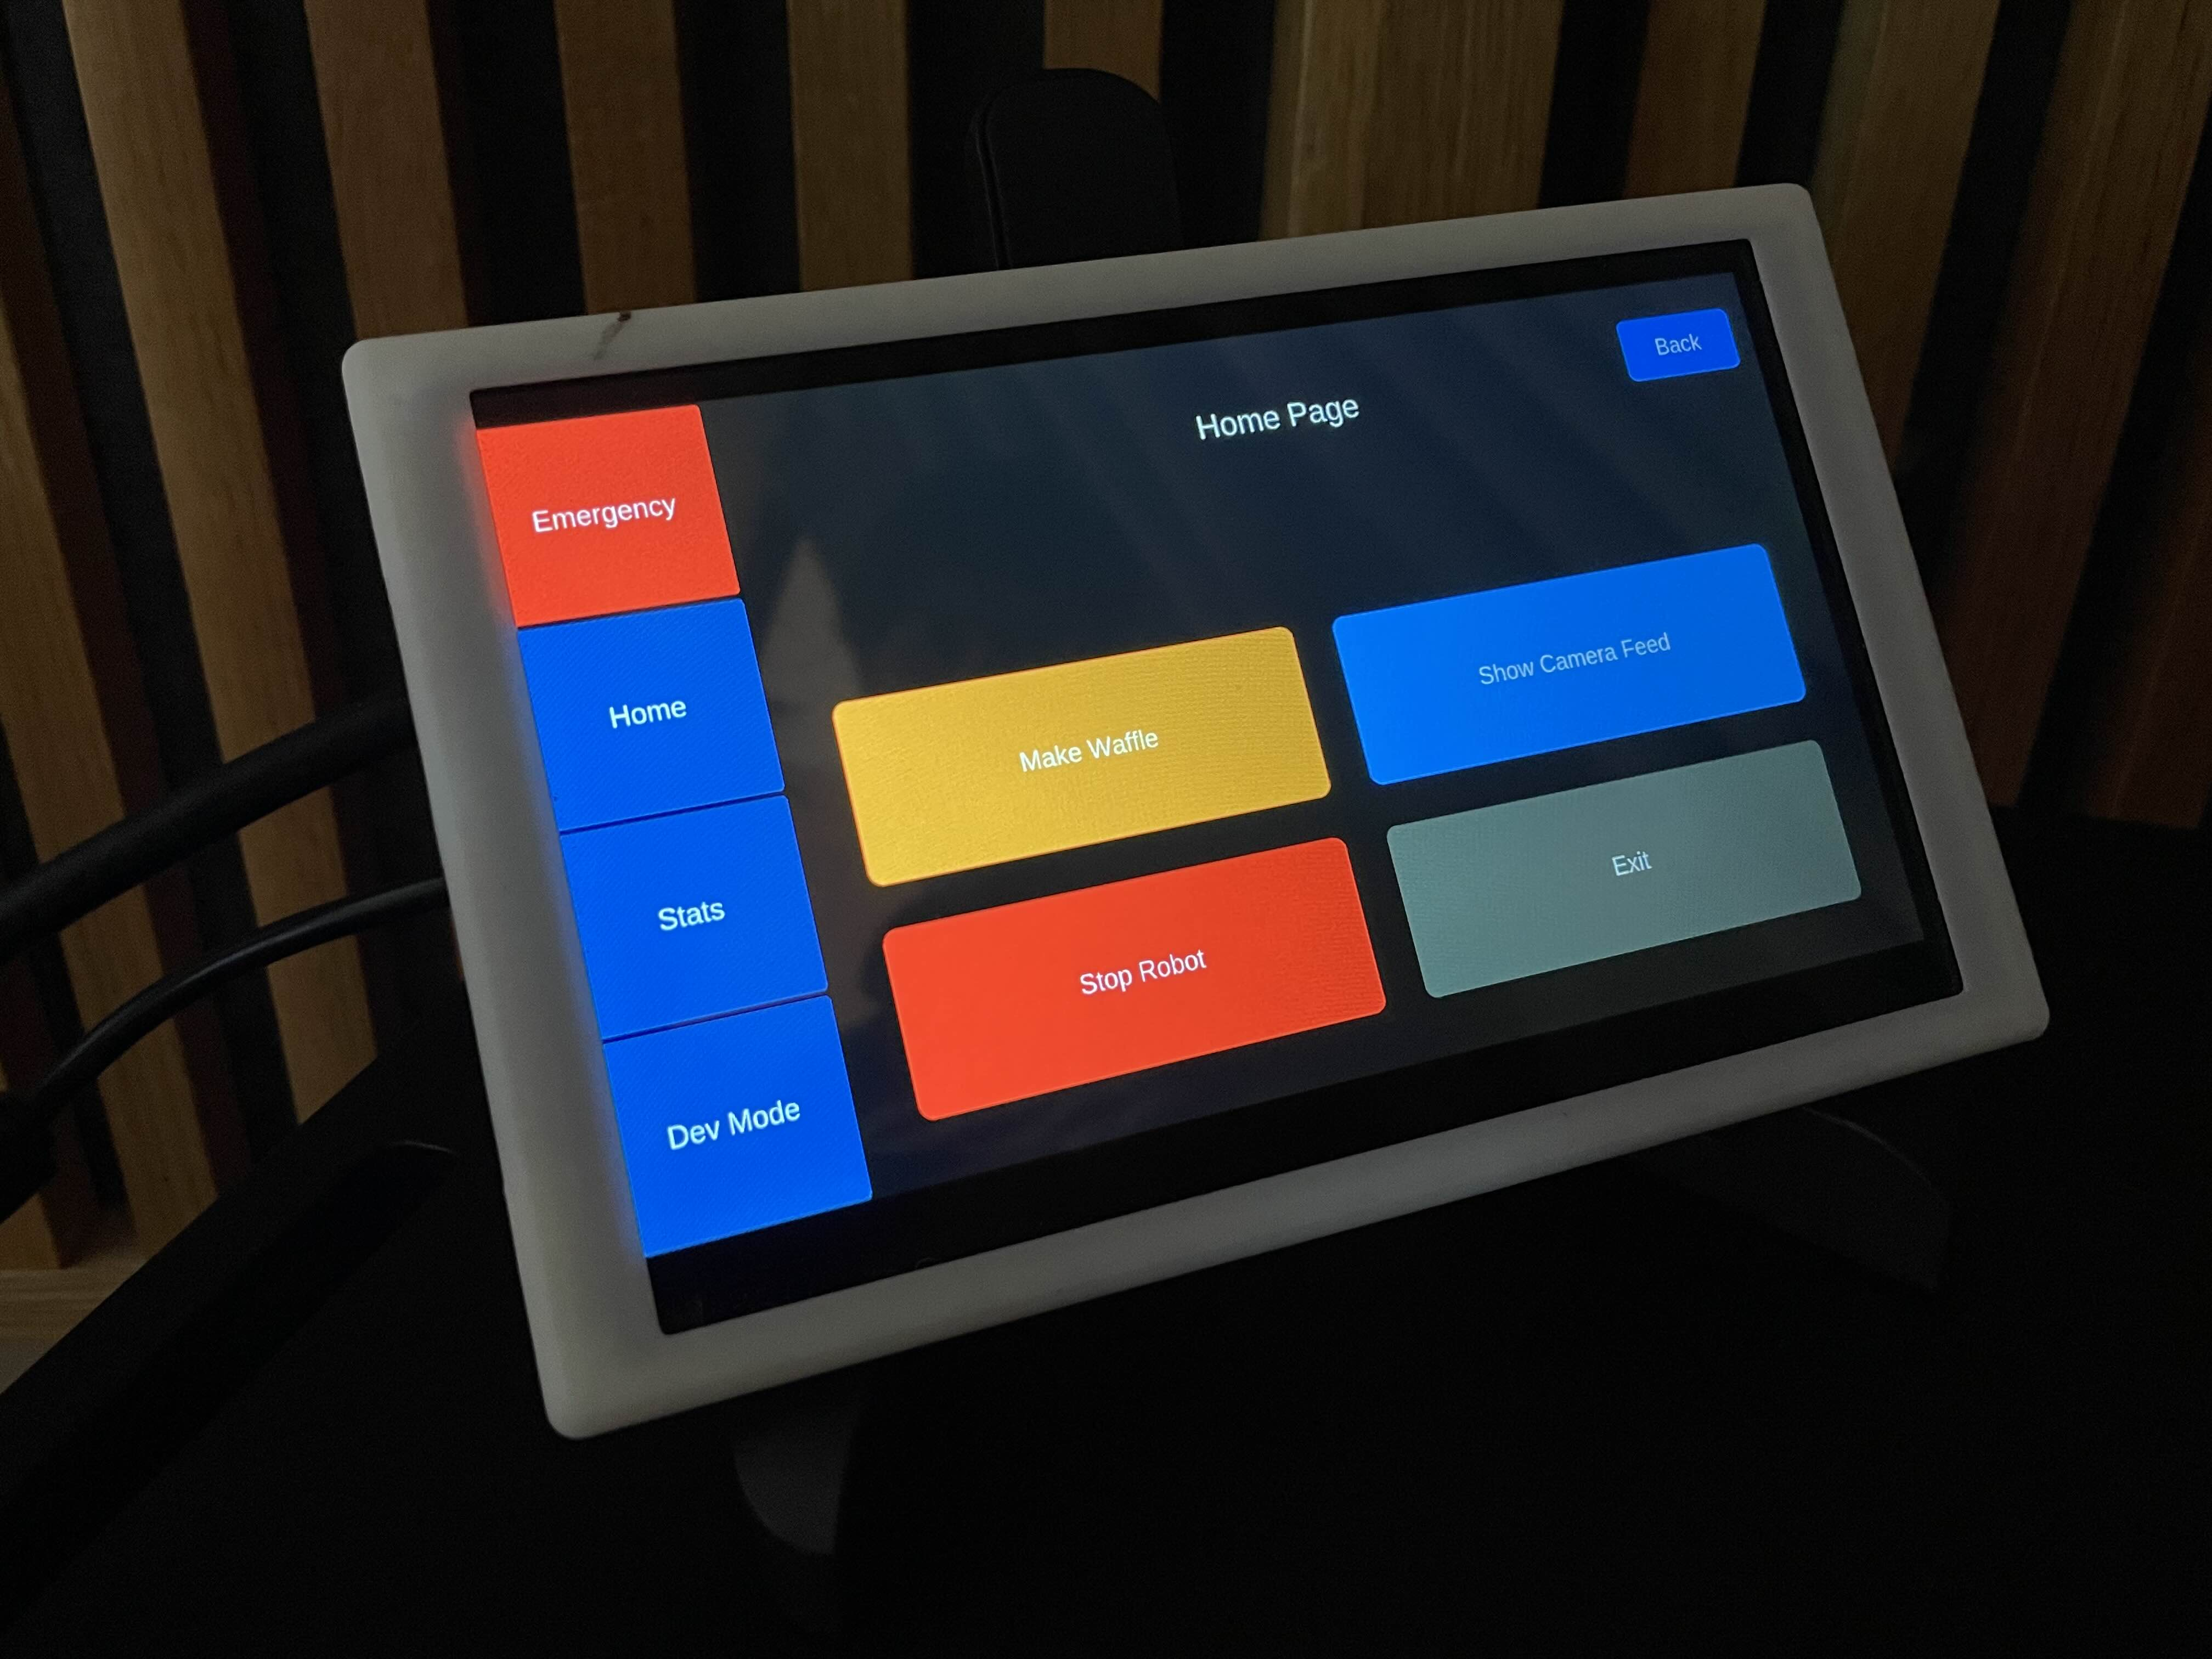
\includegraphics[width=1\linewidth]{figures/screen.jpg} 
    \caption{Ingcool 7IP-CAPLCD 7-inch touchscreen display}
    \label{fig:touchscreen}
\end{figure} 
